% Drawing 122/01-6 -- folder 122, batch 01, archive page 16 (PDF page 17).
% Transcription: au-dessous, second diagramme en perspective, sur les lettres correspondantes : $V'$ et $V'_s$ en haut, $X'_{\eta}$, $V'_s$, $t$, $e$ au milieu, $X'_{\eta}$, $V'_s \times \eta$, $V'_s$, $\eta$, $(s,t)$, $t$ en bas, reliées par des flèches montantes épaisses ; un cadre en traits doubles et un cadre au crayon ; à droite, un quadrilatère hachuré.
% Kind: arrow diagram in perspective (lattice of inclusions), with frames and a hatched region. Method 2 (schematic redraw from the facsimile). Status: ok.
% Notes: The letters are placed as on the page and the arrows drawn between the places where they start and end. A frame of heavy and double strokes runs round X'_eta and V'_s x eta; a thin pencil quadrilateral lies under the lower X'_eta and V'_s; at the right a small quadrilateral is hatched, with an arrow from its upper right corner. Left out: the node at the top left, blotted out in ink (two arrows end on it; they are drawn); the letter at the far right, struck (it reads V'_s or X'_s) and the small round letter beside the hatched quadrilateral (e or a zero); the small s at the left is drawn although it looks struck. Partial: hooks and tildes on several arrows are not drawn (the arrows V'_s to V'_s at the top right and e to t carry a tilde; the second is drawn as a plain stroke); which letter each arrow joins is read from its direction; frames and hatching are placed by eye. Overlaid 2026-11-12 (Opus 5.5) on a 400 dpi colour render: letters, arrows, frames and the two quadrilaterals match the page within about a unit; nothing corrected. Redrawn 2026-11-12 (issue 128): to check again. 2026-11-13, Claude Opus 5.5, overlay check (issue 147): not compiled (no TeX in the session); the TikZ rasterised and laid over the 236 ppi colour scan (rendered at 350 dpi), with an ink/pencil separation of the crop. Redrawn element by element on the scan (letters, arrows and frames were up to 3 units off): the eighteen arrows between the points where their ink starts and ends, with what they carry: the hooked tail of X'_eta to V' (a U), of V'_s to V' (a U) and of e to V'_s (a short upturn), the tilde over the tail of the arrow up to the upper right V'_s, and the arrow from e to t with its hooked head and the tilde stroke above it; the frame: the heavy upper left side with a thin stroke inside it, the upper right side heavy with two thin strokes beside it (the double stroke), the heavy lower sides meeting under V'_s x eta; the pencil quadrilateral (its place was right) with the two short pencil strokes across its lower left side; the hatched quadrilateral with its two heavy sides, its thin upper left side and six strokes across it, the chevron at its upper right corner and the closed loop beside it (the small round letter, e or a zero, unread, drawn as the loop it is); the struck letter at the far right (V'_s or X'_s), its prime and subscript, and the stroke through it, in the struck style as decided in #146; three small unread marks (two beside the frame's right corner, one at the far left) drawn as strokes. Every element lies on the ink to within about 1 unit. Left out: the node at the top left, blotted out in ink (a crossing-out, not part of the figure; the two arrows that end on it are drawn).
% Coordinates: 1 unit = 1 mm = 1/100 of the crop width (bbox in page fractions: [0.32, 0.42, 0.72, 0.56]).
% Redrawn by Claude (claude-fable-5-2), issue #128, 2026-11-12; not checked by a human; not compiled (no TeX in the session).
% Overlaid by Claude (claude-opus-5-5) 2026-11-12 (issue #128): rasterised from its own coordinates over the colour facsimile and checked or corrected. Not compiled. Status: partial.
% Revised by Claude Opus 5.5 (claude-opus-5-5), issue #147, 2026-11-13: overlay check on the colour scan; not checked by a human; not compiled (no TeX in the session).
% Rights: reproduces part of the work -- behind RENDER_TRANSCRIPTS, never published by itself.
\documentclass[tikz,border=3pt]{standalone}
\usepackage{amsmath,amssymb}
\usetikzlibrary{patterns,arrows.meta}
\tikzset{pencil/.style={black!45}, struck/.style={black!35}, mpt/.style={circle,draw,inner sep=1.3pt}, pt/.style={circle,fill,inner sep=0.9pt}, opt/.style={circle,draw,fill=white,inner sep=1.1pt}}
\begin{document}
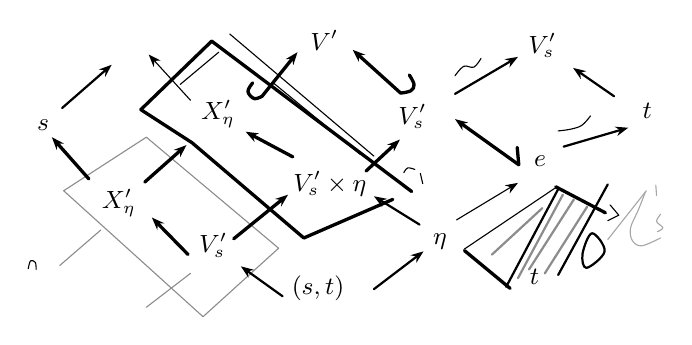
\begin{tikzpicture}[x=1mm,y=1mm,line cap=round,line join=round,font=\scriptsize]
% letters
\node[inner sep=1pt] at (6.6,-17.6) {\small $s$};
\node[inner sep=1pt] at (28.8,-16.1) {\small $X'_{\eta}$};
\node[inner sep=1pt] at (42.3,-6.8) {\small $V'$};
\node[inner sep=1pt] at (53.5,-16.5) {\small $V'_s$};
\node[inner sep=1pt] at (70,-7.5) {\small $V'_s$};
\node[inner sep=1pt] at (83.3,-15.7) {\small $t$};
\node[inner sep=1pt] at (69.7,-22.2) {\small $e$};
\node[inner sep=1pt] at (16.2,-27.4) {\small $X'_{\eta}$};
\node[inner sep=1pt] at (43,-25) {\small $V'_s \times \eta$};
\node[inner sep=1pt] at (28.2,-32.8) {\small $V'_s$};
\node[inner sep=1pt] at (57,-32.3) {\small $\eta$};
\node[inner sep=1pt] at (41.5,-38.3) {\small $(s,t)$};
\node[inner sep=1pt] at (69,-36.8) {\small $t$};
% frame of heavy and double strokes round X'_eta and V'_s x eta
\draw[very thick] (19,-15.6) -- (28,-6.9);
\draw (24,-12.4) -- (28.9,-8.3);
\draw[very thick] (28,-6.9) -- (53.4,-26);
\draw (30.3,-6) -- (48.6,-21.5);
\draw (35.7,-12.1) -- (46.9,-21.3);
\draw[very thick] (19,-15.6) -- (25.5,-19.8) -- (39.7,-31.9);
\draw[very thick] (39.7,-31.9) -- (51,-27);
% pencil quadrilateral and the two short pencil strokes across its lower left side
\draw[pencil] (9.2,-25.9) -- (19.7,-19.1) -- (36.5,-33.2) -- (26.9,-41.9) -- cycle;
\draw[pencil] (8.7,-35.4) -- (13.9,-30.9);
\draw[pencil] (19.7,-40.7) -- (25.3,-36.4);
% arrows
\draw[-{Stealth[length=1.6mm]},thick] (9,-15.4) -- (15.3,-9.9);
\draw[-{Stealth[length=1.6mm]}] (25.3,-14.4) -- (20,-8.6);
\draw[-{Stealth[length=1.6mm]},very thick] (12.4,-24.4) -- (7.7,-19.1);
\draw[very thick] plot[smooth, tension=0.6] coordinates {(33.2,-12.2) (32.6,-13.3) (33.4,-14.2) (34.4,-13.9)};
\draw[-{Stealth[length=1.6mm]},very thick] (34.4,-13.9) -- (38.9,-8.3);
\draw[-{Stealth[length=1.6mm]},very thick] (52,-13.5) -- (45.9,-8);
\draw[very thick] plot[smooth, tension=0.6] coordinates {(52,-13.5) (53.3,-13.2) (53.7,-12.4) (53.1,-11.2)};
\draw[-{Stealth[length=1.6mm]},thick] (58.9,-13.6) -- (66.9,-8.9);
\draw plot[smooth, tension=0.6] coordinates {(58.9,-11.3) (60,-10.1) (61.3,-10.2) (62.2,-9.1)};
\draw[-{Stealth[length=1.6mm]},thick] (79.1,-13.9) -- (73.9,-10.3);
\draw[-{Stealth[length=1.6mm]},thick] (72.7,-20.3) -- (80.9,-17.9);
\draw plot[smooth, tension=0.6] coordinates {(72,-18.3) (73.5,-18.1) (75,-17.6) (76.1,-16.4)};
\draw[-{Stealth[length=1.6mm]},very thick] (67,-22.6) -- (58.9,-16.8);
\draw[very thick] (67,-22.6) -- (66.8,-20.4);
\draw[-{Stealth[length=1.6mm]},very thick] (19.5,-24.8) -- (24.8,-20.1);
\draw[-{Stealth[length=1.6mm]},very thick] (25,-34) -- (20.4,-29.3);
\draw[-{Stealth[length=1.6mm]},very thick] (30.8,-32) -- (37.7,-26.4);
\draw[-{Stealth[length=1.6mm]},very thick] (38.3,-21.6) -- (32.3,-18.4);
\draw[-{Stealth[length=1.6mm]},very thick] (47.6,-23.4) -- (51.9,-19.4);
\draw[-{Stealth[length=1.6mm]},thick] (54.4,-30.2) -- (48.6,-26.6);
\draw[-{Stealth[length=1.6mm]}] (59.1,-29.6) -- (66.9,-24.9);
\draw[-{Stealth[length=1.6mm]},thick] (37,-39.3) -- (31.7,-35.5);
\draw[-{Stealth[length=1.6mm]},thick] (48.6,-38.4) -- (54.9,-33.6);
% hatched quadrilateral, its strokes, the chevron at its upper right corner and the loop beside it
\draw[very thick] (60.1,-33.5) -- (65.9,-38.3);
\draw[very thick] (71.7,-25.4) -- (78,-28.7);
\draw (60.1,-33.3) -- (71.7,-25.5);
\draw[pencil,thick] (63.6,-34) -- (70,-28.1);
\draw[thick] (65.4,-38.1) -- (72,-25.7);
\draw[pencil,thick] (66.9,-37) -- (72.6,-26.4);
\draw[pencil,thick] (68.3,-35.9) -- (74,-27);
\draw[pencil,thick] (70.3,-36.4) -- (75.7,-27.9);
\draw[thick] (72,-36.6) -- (78.3,-25.1);
\draw (78.6,-27.7) -- (79.7,-29) -- (78.3,-29.7);
\draw[thick] plot[smooth cycle, tension=0.6] coordinates {(76.3,-31.3) (77.9,-33.6) (75.6,-35.7) (75.1,-33.9)};
% struck letter at the far right, with its strike
\draw[struck] plot[smooth, tension=0.55] coordinates {(83.1,-26) (82.2,-28.3) (81.2,-30.6) (81.4,-32.2) (82.6,-32.9) (85,-31.9)};
\draw[struck] (84.4,-25.2) -- (84.5,-26.5);
\draw[struck] plot[smooth, tension=0.6] coordinates {(85,-28.9) (84.5,-29.8) (85.3,-30.6) (84.6,-31.1)};
\draw[struck] (78.3,-32.1) -- (83.2,-25.9);
% small unread marks: two right of the frame's right corner, one at the far left
\draw plot[smooth, tension=0.6] coordinates {(52.4,-23.6) (52.9,-23) (53.8,-23.2)};
\draw (54.5,-23.7) -- (54.8,-25);
\draw plot[smooth, tension=0.6] coordinates {(4.7,-35.8) (5,-34.8) (5.6,-35) (5.7,-35.9)};
\end{tikzpicture}
\end{document}
